\section{Equilibrium geometry and the universal ceiling}\label{sec:geometry}

\subsection{Rational parametrization}
Let \(x\) denote the vector of all \(q+2m+2\) concentrations, \(H(x)\) the mass-action vector
field of \eqref{eq:source}, and \(\cT\) the linear map \(x\mapsto(\ET,\FT,\ST)\) of
\eqref{eq:totals}. At an equilibrium the complex equations give
\begin{equation}\label{eq:complexes}
 C_e=p_e\,E\,S_{\tl e},\qquad Y_e=q_e\,F\,S_{\hd e},
\end{equation}
so the catalytic fluxes are \(c_eC_e=k_e^+ES_{\tl e}\) and \(\gamma_eY_e=k_e^-FS_{\hd e}\). It
is convenient to use the \emph{retained pools}
\begin{equation}\label{eq:pools}
 Z_I=S_I+\sum_{\tl e=I}C_e+\sum_{\hd e=I}Y_e ,\qquad \sum_IZ_I=\ST ,
\end{equation}
because \(\dot Z_I\) contains only catalytic fluxes. Let \(U\) and \(V\) be the \(q\times q\)
generator matrices of the upward and downward effective rates: \(U_{\hd e,\tl e}=k_e^+\),
\(V_{\tl e,\hd e}=k_e^-\), with diagonal entries making all column sums zero. With \(u=E/F\),
substituting \eqref{eq:complexes} into \(\dot Z=0\) gives
\begin{equation}\label{eq:frozen}
 F\,(uU+V)\,S=0 .
\end{equation}
For \(u>0\) the matrix \(uU+V\) is the generator of an irreducible Markov chain on the cube.
By the matrix-tree theorem \cite{MirzaevGunawardena2013,ThomsonGunawardena2009b} its kernel is
spanned by the vector \(\tau(u)\) of \emph{tree weights}: \(\tau_I(u)\) is the sum, over
spanning trees directed towards \(I\), of the products of the edge labels \(uk_e^+\) (upward)
and \(k_e^-\) (downward). Hence \(S_I=s\,\tau_I(u)\) with a scalar \(s>0\). A tree directed
towards a vertex of level \(|I|=k\) contains at least \(k\) upward edges, on the path from
\(\varnothing\), and at least \(n-k\) downward edges, on the path from \([n]\). Therefore
\(\tau_I\) is a polynomial in \(u\) with nonnegative coefficients,
\begin{equation}\label{eq:degrees}
 u^{|I|}\mid\tau_I,\qquad \deg\tau_I\le q-1-n+|I| ,\qquad \tau_\varnothing(0)>0 .
\end{equation}
Define
\begin{equation}\label{eq:ABD}
 A(u)=\sum_I\tau_I,\qquad B(u)=\sum_ep_e\tau_{\tl e},\qquad
 D(u)=\frac1u\sum_eq_e\tau_{\hd e},
\end{equation}
polynomials with \(\deg A\le q-1\), \(\deg B,\deg D\le q-2\) and \(A(0),B(0)>0\). Then
\(\sum_eC_e=sEB\) and \(\sum_eY_e=sFuD\), and the three totals read
\begin{equation}\label{eq:threetotals}
 \ET=uF(1+sB),\qquad \FT=F(1+suD),\qquad \ST=sA+suF(B+D).
\end{equation}
Write \(r=\ET/\FT\), \(L=B-rD\) and \(M=B-uD=L+(r-u)D\). Dividing the first two equations of
\eqref{eq:threetotals} gives \(su\,L(u)=r-u\). Hence, when \(u\ne r\), necessarily
\(L(u)\ne0\) and
\begin{equation}\label{eq:reconstruct}
 s=\frac{r-u}{uL(u)},\qquad F=\frac{\FT L(u)}{M(u)},\qquad E=uF ,
\end{equation}
and the state is determined by \(u\). An equilibrium requires \(s>0\) and \(F>0\), that is,
\(L(u)\), \(M(u)\) and \(r-u\) have the same sign. Inserting \eqref{eq:reconstruct} into the
third equation of \eqref{eq:threetotals} and multiplying by \(uLM\) yields, after an
elementary rearrangement, the \emph{eliminant}
\begin{equation}\label{eq:elim}
 \cP(u)=(\ST-\ET-\FT)\,uLM-(r-u)\,AM+(u+1)\,\FT\,uL^2=0 .
\end{equation}

\begin{proposition}[Equilibrium count]\label{prop:count}
For all positive rates and totals, every positive equilibrium has a ratio \(u=E/F\) that is a
positive root of \(\cP\), distinct equilibria have distinct ratios, \(\cP\) has degree at most
\(2q-1\) and \(\cP(0)<0\). Hence every compatibility class contains at most \(2^{n+1}-1\)
positive equilibria.
\end{proposition}
\begin{proof}
The degree bound follows from \eqref{eq:ABD}, and
\(\cP(0)=-rA(0)M(0)=-rA(0)B(0)<0\), so \(\cP\not\equiv0\). For \(u\ne r\) the claims were
shown above. Suppose there is an equilibrium with \(u=r\). Then \(L(r)=0\), so \(M(r)=0\) and
\(\cP(r)=0\). With \(u=r\) the first two totals coincide and give \(F=\FT/(1+srD(r))\), and
the substrate total becomes
\(sA(r)+\FT\,sr\,(B(r)+D(r))/(1+srD(r))\), which is strictly increasing in \(s\) from \(0\) to
\(\infty\). So there is exactly one equilibrium with this ratio, and it is a root of \(\cP\).
\end{proof}

\begin{remark}
The separate treatment of \(u=r\) matters: a reconstruction formula with a vanishing
denominator is not an exclusion proof. For the sequential chain the same elimination gives a
polynomial of degree \(2n+1\); the sharper Wang--Sontag bound \(2n-1\) uses the special
structure \(\tau_i=t_iu^i\) \cite{WangSontag2008}. We do not know whether \(2^{n+1}-1\) is
attained on the cube. The example of Section~\ref{sec:example} has \(n=3\), \(\deg\cP=15\), and
seven positive equilibria.
\end{remark}

\subsection{Regular totals at fixed rates}
The next lemma is the technical core of the two upper bounds. It produces nondegenerate
equilibria by perturbing only the \emph{totals}. Perturbing rates, which is the usual device,
would destroy square balance and could not be used in Section~\ref{sec:balance}.

\begin{lemma}[Regularity with fixed rates]\label{lem:regular}
Fix positive rates. \textup{(i)} At every positive \(x\), the derivative \(DH(x)\) has rank
\(d=q+2m-1\). \textup{(ii)} The set \(\cZ\) of positive equilibria of all classes is a
three-dimensional embedded submanifold, parametrized by
\((u,s,F)\in\R^3_{>0}\) through \(S=s\tau(u)\), \(E=uF\) and \eqref{eq:complexes}, and
\(T_x\cZ=\ker DH(x)\) for \(x\in\cZ\). \textup{(iii)} A point \(x\in\cZ\) is a regular point of
the restricted total map \(\cT|_\cZ:\cZ\to\R^3\) if and only if the Jacobian of \(H\) restricted
to the class through \(x\) is nonsingular. \textup{(iv)} The totals for which some equilibrium
in the class is degenerate form a set of Lebesgue measure zero in \(\R^3_{>0}\).
\end{lemma}
\begin{proof}
(i) The image of \(H\) lies in \(\ker\cT\), which has dimension \(d\), so the rank is at most
\(d\). For the lower bound select the \(2m\) equations for \(\dot C_e,\dot Y_e\) and the
\(q-1\) equations for \(\dot Z_I\), \(I\ne\varnothing\) (linear combinations of the rows of
\(DH\)), and the \(2m\) complex columns together with the columns of \(S_I\),
\(I\ne\varnothing\). Since \(\dot Z\) depends only on the complexes, the selected
\(d\times d\) matrix has the block form
\(\bigl(\begin{smallmatrix}-\Delta&\Pi\\ \Gamma&0\end{smallmatrix}\bigr)\), where
\(\Delta=\diag(b_e+c_e,\beta_e+\gamma_e)\) is positive, \(\Pi\) contains the entries
\(a_eE\) and \(\alpha_eF\) in the columns of \(S_{\tl e}\) and \(S_{\hd e}\), and \(\Gamma\)
contains the catalytic constants with the signs of \(\dot Z\). Its determinant is
\(\det(-\Delta)\det(\Gamma\Delta^{-1}\Pi)\), and \(\Gamma\Delta^{-1}\Pi\) is the matrix
\(EU+FV=F(uU+V)\) with the row and the column of \(\varnothing\) deleted. By the matrix-tree
theorem this principal minor equals \(\pm F^{q-1}\tau_\varnothing(u)\ne0\).

(ii) The parametrization is smooth and injective, with smooth inverse
\(u=E/F\), \(s=S_\varnothing/\tau_\varnothing(E/F)\), and by the discussion preceding
\eqref{eq:degrees} it covers \(\cZ\). Differentiating \(H=0\) along it gives
\(T_x\cZ\subseteq\ker DH(x)\), and both spaces have dimension three by (i).

(iii) \(D(\cT|_\cZ)(x)\) is an isomorphism if and only if \(T_x\cZ\cap\ker\cT=0\), that is,
\(\ker DH(x)\cap\ker\cT=0\), which says that \(DH(x)\) is injective on the tangent space
\(\ker\cT\) of the class. (iv) is Sard's theorem \cite{Milnor1965} for the smooth map
\(\cT|_\cZ\) between three-dimensional manifolds.
\end{proof}

\subsection{Degree and the index of a sink}
\begin{lemma}[Boundary and degree]\label{lem:degree}
For positive totals, the compatibility class contains no equilibrium on its
relative boundary. If all equilibria in the class are nondegenerate, they are finite in
number, and
\begin{equation}\label{eq:degree}
 \sum_{x^*}\ind(x^*)=1,\qquad \ind(x^*)=\sign\det\bigl(-J(x^*)\bigr),
\end{equation}
where \(J\) is the Jacobian restricted to the class.
\end{lemma}
\begin{proof}
Let \(x\) be an equilibrium in the class. If \(E=0\), then \(\dot C_e=-(b_e+c_e)C_e=0\) for
all \(e\), so \(\ET=0\), a contradiction; hence \(E,F>0\). If every \(S_I\) vanished, the
complex equations would give \(C_e=Y_e=0\) and \(\ST=0\). Thus \(S\ne0\) is a nonnegative
solution of \eqref{eq:frozen} with an irreducible generator, so \(S>0\), and then all
complexes are positive by \eqref{eq:complexes}. The class is compact and convex, and \(H\)
points inward or is tangent on each face \(\{x_i=0\}\). For an interior point \(x_0\), the
homotopy \((1-t)(-H(x))+t(x-x_0)\) has no zero on the boundary: for \(0<t<1\) a zero would
satisfy \(H_i(x)=\tfrac{t}{1-t}(x-x_0)_i<0\) on some face \(x_i=0\), and \(t=0\) is excluded by
the first part. Hence the Brouwer degree of \(-H\) on the interior of the class is one
\cite{Deimling,Hofbauer1990}. Nondegenerate equilibria are isolated, and they cannot
accumulate in the compact class because the limit would be a nonisolated equilibrium in its
interior. The degree is the sum of their indices.
\end{proof}

\begin{lemma}[Index of a sink]\label{lem:index}
A sink is an isolated equilibrium of its class, and the index of \(-H\) at a sink is \(+1\),
whether or not the sink is hyperbolic.
\end{lemma}
\begin{proof}
All trajectories starting near a sink converge to it, so no other equilibrium is nearby. For
the index, take a compact ball \(N\) in the basin. For large \(t\) the time-\(t\) map
\(\varphi_t\) sends \(N\) into its interior, so the fixed-point index of \(\varphi_t\) on \(N\)
is one; since no point of \(\partial N\) is periodic, the homotopy \(t\downarrow0\) transfers
this to the index of \(-H\). This is the classical theorem of Krasnosel'ski\u{\i} on
asymptotically stable equilibria \cite{KrasnoselskiiZabreiko}; see also \cite{Companion}.
\end{proof}

\begin{theorem}[Universal ceiling]\label{thm:upper}
For all positive rates and totals, the class contains at most \(2^n\) sinks. Thus \(C_n\le2^n\).
\end{theorem}
\begin{proof}
First let the totals be regular in the sense of Lemma~\ref{lem:regular}(iv). Let \(p_+\) and
\(p_-\) be the numbers of equilibria of index \(+1\) and \(-1\). Then \(p_+-p_-=1\) by
\eqref{eq:degree} and \(p_++p_-\le2q-1\) by Proposition~\ref{prop:count}, so \(p_+\le q\).

For arbitrary totals \(c\), suppose there were \(q+1\) sinks. Eliminate \(S_\varnothing,E,F\)
by \eqref{eq:totals}; this identifies all nearby classes with open subsets of one space
\(\R^d\) (the \emph{class chart}) on which the field depends continuously on the totals.
Choose disjoint compact neighbourhoods \(N_1,\dots,N_{q+1}\) of the sinks, inside the positive
class, each containing no other equilibrium. By Lemma~\ref{lem:index} the degree of \(-H\) on
each \(N_i\) is one. For totals \(c'\) close to \(c\) the field has no zero on
\(\partial N_i\) and the degrees are unchanged. By Lemma~\ref{lem:regular} we may take \(c'\)
regular; then every \(N_i\) contains an equilibrium of index \(+1\), so \(p_+\ge q+1\), a
contradiction.
\end{proof}

\section{Square balance and the sequential ceiling}\label{sec:balance}

\subsection{Compression of a balanced cube to a chain}
Assume \eqref{eq:balance-intro}. Any two monotone paths from \(\varnothing\) to \(I\) differ by
a sequence of swaps of adjacent site additions, and each swap leaves the product of the ratios
\(\rho_e\) along the path unchanged. Hence there are positive weights with
\begin{equation}\label{eq:weights}
 w_\varnothing=1,\qquad w_{\hd e}=\rho_e\,w_{\tl e}\quad\text{for every edge }e .
\end{equation}
Then \(S_I=s\,w_Iu^{|I|}\) satisfies \(uk_e^+S_{\tl e}=k_e^-S_{\hd e}\) on every edge, so it
solves \eqref{eq:frozen}, and by irreducibility \(\tau_I(u)\) is proportional to
\(w_Iu^{|I|}\): at a balanced equilibrium every edge carries zero net effective flux. Group the
weights by level,
\begin{equation}\label{eq:levels}
 A_k=\sum_{|I|=k}w_I,\qquad B_k=\sum_{|\tl e|=k}p_ew_{\tl e},\qquad
 D_k=\sum_{|\hd e|=k+1}q_ew_{\hd e}\qquad(0\le k\le n-1),
\end{equation}
and \(A_n=w_{[n]}\). After division by the common factor, \(A=\sum_kA_ku^k\),
\(B=\sum_kB_ku^k\) and \(D=\sum_kD_ku^k\).

\begin{lemma}[Compression]\label{lem:compression}
Let the cube rates be square balanced. The sequential chain with loadings, effective rates and
catalytic constants
\[
 \bar p_{k+1}=\frac{B_k}{A_k},\qquad \bar q_{k+1}=\frac{D_k}{A_{k+1}},\qquad
 \bar c_{k+1}=\frac{D_k}{B_k},\qquad \bar\gamma_{k+1}=1\qquad(0\le k\le n-1),
\]
and any positive dissociation constants, has tree weights \(A_ku^k\) and the same polynomials
\(A,B,D\). Consequently, for every triple of totals, \((u,s,F)\mapsto(u,s,F)\) is a bijection
between the positive equilibria of the cube and those of the chain.
\end{lemma}
\begin{proof}
The effective ratio of the chain at step \(k+1\) is
\(\bar c_{k+1}\bar p_{k+1}/(\bar\gamma_{k+1}\bar q_{k+1})=A_{k+1}/A_k\), which gives the tree
weights \(A_ku^k\), and then \(\sum_k\bar p_{k+1}A_ku^k=B\) and
\(\sum_k\bar q_{k+1}A_{k+1}u^{k}=D\). The equations \eqref{eq:threetotals}, which determine the
equilibria, involve the network only through \(A,B,D\). Association constants
\(\bar a=\bar p(\bar b+\bar c)\) and \(\bar\alpha=\bar q(\bar\beta+\bar\gamma)\) realize the
loadings.
\end{proof}
The lemma is a statement about equilibria. It does not assert that the dynamics of the
balanced cube reduces to that of the chain, and in general it does not.

\subsection{The symmetric lift}
Under a stronger hypothesis the reduction is exact. Let a chain have the rate
constants \(a_k,b_k,c_k,\alpha_k,\beta_k,\gamma_k\) for \(1\le k\le n\). Its \emph{symmetric
lift} to the cube is defined by
\begin{equation}\label{eq:lift}
 a_e=\frac{a_{k+1}}{n-k},\quad \alpha_e=\frac{\alpha_{k+1}}{k+1},\quad
 (b_e,c_e,\beta_e,\gamma_e)=(b_{k+1},c_{k+1},\beta_{k+1},\gamma_{k+1})
 \quad\text{if }|\tl e|=k .
\end{equation}
The lifted ratios \(\rho_e\) depend only on the level, so the lift is square balanced. Let
\(\Pi\) be the aggregation map that sums the \(S_I\) over each level and the \(C_e\) and
\(Y_e\) over all edges with tails at the same level.

\begin{proposition}[Exact deterministic reduction]\label{prop:lift}
For the symmetric lift, \(\Pi x(t)\) together with \(E,F\) solves the mass-action equations of
the chain with the same totals. The positive equilibria of the cube are exactly the uniform
lifts of those of the chain; an equilibrium of the cube is a sink if and only if the
corresponding equilibrium of the chain is, and hyperbolic sinks correspond to hyperbolic
sinks.
\end{proposition}
\begin{proof}
A vertex of level \(k\) has \(n-k\) upward and \(k\) downward edges, so
\(\sum_{|\tl e|=k}a_eES_{\tl e}=a_{k+1}E\sum_{|I|=k}S_I\) and
\(\sum_{|\hd e|=k+1}\alpha_eFS_{\hd e}=\alpha_{k+1}F\sum_{|I|=k+1}S_I\); all other terms are
linear with level-dependent constants. This gives the first claim. Collect the \(q+2m\)
substrate-carrying species in a vector \(z\). Then \(\dot z=\mathcal A(E,F)z\), where, for
\(E,F>0\), \(\mathcal A\) is the generator of an irreducible Markov chain describing the fate of
one substrate molecule, and \(E,F\) depend on \(z\) only through \(y=\Pi z\). Let \(\Theta\) be
the uniform lift, \(\Pi\Theta=I\). The symmetry of \eqref{eq:lift} gives
\(\Pi\mathcal A=\bar{\mathcal A}\Pi\) and \(\mathcal A\Theta=\Theta\bar{\mathcal A}\), where
\(\bar{\mathcal A}\) is the corresponding matrix of the chain. Hence \(w=z-\Theta\Pi z\)
satisfies \(\dot w=\mathcal A(E,F)w\) on the invariant subspace \(\ker\Pi\), while \(y\) is
autonomous. The null vector of \(\mathcal A\) is positive and therefore not in \(\ker\Pi\), so
\(\mathcal A|_{\ker\Pi}\) is Hurwitz. Thus every equilibrium has \(w=0\); the Jacobian is block
triangular with blocks \(\bar J\) and \(\mathcal A|_{\ker\Pi}\); and asymptotic stability of
\(y^*\) implies that of \((y^*,0)\), because \(w\) obeys a linear equation whose coefficient
matrix converges to a Hurwitz matrix. The converse holds because \(\{w=0\}\) is invariant.
\end{proof}

\subsection{Proof of Theorem~\ref{thm:balanced}}
Let the rates be square balanced. By Lemma~\ref{lem:compression} and the Wang--Sontag theorem
\cite[Theorem~3]{WangSontag2008}, every class contains at most \(2n-1\) positive equilibria.
At regular totals, \eqref{eq:degree} gives \(p_+-p_-=1\) and \(p_++p_-\le2n-1\), so
\(p_+\le n\). Now repeat the second half of the proof of Theorem~\ref{thm:upper}: if some class
had \(n+1\) sinks, nearby regular totals, \emph{for the same balanced rates}, would give
\(p_+\ge n+1\). This is where Lemma~\ref{lem:regular} is needed in the form stated. For
attainment, \cite[Theorem~1.1]{Companion} provides a chain with \(n\) hyperbolic sinks
(Appendix~\ref{app:sequential}), and by Proposition~\ref{prop:lift} its symmetric lift has
\(n\) hyperbolic sinks.\qed

\begin{remark}[What balance does and does not mean]\label{rem:balance}
(a) Square balance is a condition on the \(2m\) effective ratios only. It does not make the
network detailed balanced: every balanced equilibrium carries the positive futile-cycle flux
\(c_eC_e=\gamma_eY_e\) on each edge. (b) The effective affinity of a square compares two
kinetic pathways between the same phosphoforms. It is not the free energy of ATP hydrolysis,
which in the reversible extension of Section~\ref{sec:driving} is the same on every edge
whatever the effective affinities are. (c) Nonzero affinity is necessary for more than \(n\)
sinks but not sufficient; in exploratory computations, squares with circulating rates and
several admissible branches did not by themselves produce additional stable branches.
\end{remark}

\section{Exponentially many sinks from unrestricted loading}\label{sec:lower}
Theorem~\ref{thm:balanced} shows that additional sinks must come from unbalanced kinetics.
This section constructs them. The idea is to separate two tasks. The \emph{effective rates}
\(k_e^\pm\) are kept near the independent-site values, which makes a one-parameter family of
saturated states normally attracting. The \emph{loadings} \(p_e,q_e\), which can be varied
without changing the effective rates, are then used to program the slow drift along this
family. The loadings enter linearly, and their span has dimension at least \(2^{n-2}+n\).

\subsection{The loading space and its positive kernel}
Fix the effective rates. By \eqref{eq:ABD} the map \((p,q)\mapsto L=B-rD\) is linear, with
image
\begin{equation}\label{eq:W}
 \cW=\spanop\bigl\{\tau_{\tl e}(u),\ \tau_{\hd e}(u)/u\ :\ e\ \text{an edge}\bigr\}.
\end{equation}
\begin{lemma}[Positive kernel]\label{lem:kernel}
For all \(u\),
\(u\sum_ek_e^+\tau_{\tl e}(u)=\sum_ek_e^-\tau_{\hd e}(u)\). Consequently
\((p,q)=(rk^+,k^-)\) lies in the kernel of \((p,q)\mapsto B-rD\), and any real solution
\((p,q)\) of \(B-rD=L\) becomes a positive solution after adding a sufficiently large multiple
of it.
\end{lemma}
\begin{proof}
Multiply the \(I\)-th row of \((uU+V)\tau=0\) by \(|I|\) and sum. Every upward transition
raises \(|I|\) by one and every downward transition lowers it by one, which gives the
identity; the rest is immediate.
\end{proof}

\begin{lemma}[Interpolation rank]\label{lem:rank}
Let \(d_0=2^{n-2}+n\) and let \(u_1<\dots<u_{d_0}\) be positive. The set of effective rates
\(k^\pm\in\R^{2m}_{>0}\) for which the evaluation map
\(\R^{2m}\to\R^{d_0}\), \((p,q)\mapsto\bigl(L(u_j)\bigr)_j\), is surjective is open and
dense. In particular it contains rational points arbitrarily close to the independent-site
rates \(k_e^+=k_e^-=1\).
\end{lemma}
\begin{proof}
A \(d_0\times d_0\) minor of the evaluation matrix is a polynomial in the effective rates, so
it suffices to find one point of the closed orthant \(\R^{2m}_{\ge0}\) where some minor is
nonzero: a polynomial that is not identically zero is nonzero on an open dense set. We use a
sparse witness in which some rates vanish but the graph remains connected, so that \(\tau\) is
still the vector of tree weights.

Split the cube into \(K=2^{n-2}\) square faces by fixing the last \(n-2\) coordinates
\(b\in\{0,1\}^{n-2}\); let \(h=|b|\) be the height of face \(b\) and call its vertex with first
two coordinates \(00\) its \emph{anchor}. Keep the four edges of each face. Join the anchors by
a spanning tree of the \((n-2)\)-cube of anchors, and set the rates of all other edges between
faces to zero (Figure~\ref{fig:cube}). On face \(b\) take upward rates \(\lambda_b(1,2,3,5)\)
and downward rates \((7,11,13,17)\) on the edges \(00\to10\), \(00\to01\), \(10\to11\),
\(01\to11\), with distinct \(\lambda_b>0\). On each tree edge take \(k^+=k^-=1\).

Removing a tree edge disconnects the graph, so its stationary net flux vanishes and the anchor
weights are in the ratios \(u^h\). Within a face the weights are those of the isolated square.
A direct computation (or the matrix-tree theorem on a \(4\)-cycle) gives, for the anchor and
the two middle vertices of the square,
\begin{equation}\label{eq:square}
 2310+1016\lambda_bu,\qquad
 \lambda_bu\,(330+195\lambda_bu),\qquad \lambda_bu\,(420+153\lambda_bu).
\end{equation}
Let \(\ell_b(u)=2310+1016\lambda_bu\) and \(Z=\prod_b\ell_b\). Up to one common factor, the
weights are \(u^hZ\) at the anchors and \(u^{h}Z\) times the last two expressions in
\eqref{eq:square} divided by \(\ell_b\) at the middle vertices. All these vertices are tails of
retained edges. Since \(330\cdot153-420\cdot195=-31410\ne0\), the two linear factors in
\eqref{eq:square} span all linear polynomials, so \(\cW\) contains \(u^{h+1}Z\) and
\(u^{h+1}Z/\ell_b\) for every face, as well as \(u^hZ\). Hence \(u^kZ\in\cW\) for
\(0\le k\le n-1\). Dividing \(u^{h+1}\) by \(\ell_b\) leaves a polynomial of degree \(h\le n-2\)
and a nonzero constant remainder, so \(Z/\ell_b\in\cW\) for every \(b\). The \(K\) polynomials
\(Z/\ell_b\) have degree \(K-1\) and are linearly independent, as evaluation at the \(K\)
distinct roots of the \(\ell_b\) shows; together with \(Z,uZ,\dots,u^{n-1}Z\) they span all
polynomials of degree at most \(K+n-1\). Evaluation of this \(d_0\)-dimensional space at
\(d_0\) distinct points is bijective, and the common factor only rescales the rows of the
evaluation matrix.
\end{proof}

\begin{figure}[tbp]
\centering
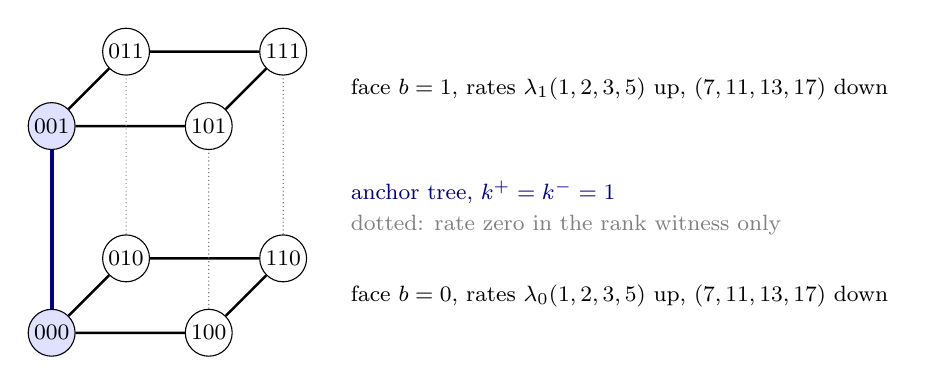
\begin{tikzpicture}[scale=1.05,every node/.style={font=\footnotesize},
  v/.style={circle,draw,inner sep=1.2pt,minimum size=15pt},
  keep/.style={line width=0.9pt},drop/.style={densely dotted,gray},
  atree/.style={line width=1.4pt,blue!55!black}]
 % face b=0
 \node[v,fill=blue!12] (a000) at (0,0) {$000$};
 \node[v] (a100) at (1.9,0) {$100$};
 \node[v] (a010) at (0.9,0.9) {$010$};
 \node[v] (a110) at (2.8,0.9) {$110$};
 % face b=1
 \node[v,fill=blue!12] (a001) at (0,2.5) {$001$};
 \node[v] (a101) at (1.9,2.5) {$101$};
 \node[v] (a011) at (0.9,3.4) {$011$};
 \node[v] (a111) at (2.8,3.4) {$111$};
 \draw[keep] (a000)--(a100) (a000)--(a010) (a100)--(a110) (a010)--(a110);
 \draw[keep] (a001)--(a101) (a001)--(a011) (a101)--(a111) (a011)--(a111);
 \draw[atree] (a000)--(a001);
 \draw[drop] (a100)--(a101) (a010)--(a011) (a110)--(a111);
 \node[anchor=west] at (3.5,0.45) {face $b=0$, rates $\lambda_0(1,2,3,5)$ up, $(7,11,13,17)$ down};
 \node[anchor=west] at (3.5,2.95) {face $b=1$, rates $\lambda_1(1,2,3,5)$ up, $(7,11,13,17)$ down};
 \node[anchor=west,blue!55!black] at (3.5,1.7) {anchor tree, $k^+=k^-=1$};
 \node[anchor=west,gray] at (3.5,1.3) {dotted: rate zero in the rank witness only};
\end{tikzpicture}
\caption{The cube of phosphoforms for \(n=3\) and the sparse witness used in the proof of
Lemma~\ref{lem:rank}. Each vertex \(I\) carries a free form \(S_I\); each edge carries the two
complexes \(C_e\) and \(Y_e\) of \eqref{eq:source}. The witness only proves that a polynomial
minor does not vanish identically; all dynamical statements use the full cube with positive
rates on every edge.}
\label{fig:cube}
\end{figure}

\subsection{A normally attracting saturated family}
For \(S\in\R^q_{>0}\) put \(A_1(S)=\sum_ek_e^+S_{\tl e}\) and \(B_1(S)=\sum_ek_e^-S_{\hd e}\),
and consider the \emph{saturated field}
\begin{equation}\label{eq:saturated}
 \frac{\dd S}{\dd\sigma}=G(S)=\frac{US}{A_1(S)}+\frac{VS}{B_1(S)} .
\end{equation}
It describes substrate processed by two fully saturated enzymes: the total upward and the
total downward flux are both equal to one. Hence \(G\) conserves \(S_0=\sum_IS_I\) and the
modification count \(\Phi(S)=\sum_I|I|S_I\).
\begin{lemma}[Normal attraction]\label{lem:normal}
\textup{(i)} For every \(S_0>0\), the equilibria of \eqref{eq:saturated} with \(\sum S_I=S_0\)
form the curve \(\Gamma=\{S_0\tau(u)/A(u):u>0\}\). \textup{(ii)} Let \(J_u\subset(0,\infty)\)
be a compact interval. For all effective rates in a neighbourhood of the independent-site
rates, depending on \(J_u\), and at every point of \(\Gamma\) with \(u\in J_u\), the
linearization of \(G\) on \(\{\sum h_I=0\}\) has a simple eigenvalue zero, with eigenvector
tangent to \(\Gamma\), and \(q-2\) eigenvalues with negative real parts, and
\(\dd\Phi/\dd u>0\) along \(\Gamma\).
\end{lemma}
\begin{proof}
(i) \(G(S)=B_1^{-1}\bigl((B_1/A_1)U+V\bigr)S\) vanishes if and only if \(S\) is proportional to
\(\tau(u')\) with \(u'=B_1(S)/A_1(S)\), and by Lemma~\ref{lem:kernel} this relation holds
identically for \(S\propto\tau(u')\). (ii) At independent-site rates,
\(A_1=nS_0-\Phi\) and \(B_1=\Phi\) are constant on each invariant slice
\(\{S_0,\Phi\ \text{fixed}\}\), on which \(G\) is therefore the linear field of the irreducible
generator \(G_0=U/A_1+V/B_1\). The row vectors \(\one^T\) and \((|I|)_I\) span a left-invariant
subspace of \(G_0\) with eigenvalues \(0\) and \(-(1/A_1+1/B_1)\), so their common kernel,
which is the tangent space of the slice, is invariant and carries the remaining \(q-2\)
eigenvalues, all with negative real parts. The stationary distribution is binomial, with
\(\Phi/S_0=nu/(1+u)\), which is increasing. The curve \(\Gamma\) is explicit for all effective
rates and depends smoothly on them, and \(\Phi\) is conserved for all of them; by continuity
of the spectrum on the compact set \(J_u\), the conclusion persists for nearby rates.
\end{proof}
The point of the lemma is that transverse stability is obtained independently of the scalar
equation that will determine the position of the equilibria along \(\Gamma\).

\subsection{Realization with retained enzymes}
Fix \(J_u=[u_1,u_{d_0}]\) and \(r>u_{d_0}\), effective rates as in Lemmas~\ref{lem:rank}
and~\ref{lem:normal}, a small \(\eta>0\), and totals \(\ET=r\eta\), \(\FT=\eta\),
\(\ST>\eta(r+1)\). For real \emph{corrections} \(v^\pm\in\R^m\), a large \(\kappa\) and a small
\(\eb>0\) define
\begin{equation}\label{eq:loading}
\begin{aligned}
 p_e&=\kappa rk_e^++v_e^+,& c_e&=k_e^+/p_e,& a_e&=p_e/\eb,& b_e&=1/\eb-c_e,\\
 q_e&=\kappa k_e^-+v_e^-,& \gamma_e&=k_e^-/q_e,& \alpha_e&=q_e/\eb,& \beta_e&=1/\eb-\gamma_e .
\end{aligned}
\end{equation}
For large \(\kappa\) and small \(\eb\) all constants are positive, the loadings are
\(p_e,q_e\) and the effective rates are \(k_e^\pm\), independently of \(\kappa\), \(v^\pm\) and
\(\eb\). In particular the \emph{equilibria} of \eqref{eq:source} do not depend on \(\eb\).

\emph{Fast binding.} As \(\eb\to0\) the binding reactions equilibrate. The fast subsystem is a
detailed-balanced mass-action system whose \(2m\) reaction vectors are linearly independent,
since each involves its own complex. In reaction-extent coordinates its linearization at the
binding equilibrium is \(-\Phi_{\!f}\,\Gamma_{\!f}^TX^{-1}\Gamma_{\!f}\), where
\(\Gamma_{\!f}\) is the fast stoichiometric matrix, \(\Phi_{\!f}\) the diagonal matrix of
equilibrium fluxes and \(X\) the diagonal matrix of concentrations; it is similar to a negative
definite matrix. Hence the manifold \eqref{eq:complexes} of binding equilibria is normally
attracting, and by the standard theory of singularly perturbed systems
\cite{Fenichel1979,KKO}, at an equilibrium the Jacobian of \eqref{eq:source} has, for small
\(\eb\), \(2m\) eigenvalues with real parts of order \(-1/\eb\) and \(q-1\) eigenvalues
converging to those of the \emph{reduced system}
\begin{equation}\label{eq:reduced}
 \dot Z=E\,US+F\,VS,\qquad
 E=\frac{r\eta}{1+\sum_ep_eS_{\tl e}},\quad F=\frac{\eta}{1+\sum_eq_eS_{\hd e}},
\end{equation}
in which \(S\) is a function of the pools \(Z\) of \eqref{eq:pools}. The map \(S\mapsto Z\) is
a local diffeomorphism: in logarithmic coordinates \(\sigma_I=\log S_I\) its derivative is
\begin{equation}\label{eq:mass}
 \bM=\diag(S+c+y)-\frac{cc^T}{\ET}-\frac{yy^T}{\FT},\qquad
 c_I=\sum_{\tl e=I}C_e,\quad y_I=\sum_{\hd e=I}Y_e ,
\end{equation}
and the Cauchy--Schwarz inequality gives
\((c^Tz)^2\le(\sum_Ic_I)\sum_Ic_Iz_I^2\le\ET\sum_Ic_Iz_I^2\), and similarly for \(y\), so
\(z^T\bM z\ge\sum_IS_Iz_I^2>0\).

\emph{Saturation.} Put \(\varepsilon=1/\kappa\) and use the time \(\sigma=\eta t/\kappa\).
Then \eqref{eq:reduced} becomes
\begin{equation}\label{eq:eps-family}
 \frac{\dd Z}{\dd\sigma}=\hat E\,US+\hat F\,VS,\qquad
 \hat E=\frac{r}{\varepsilon+rA_1(S)+\varepsilon\sum_ev_e^+S_{\tl e}},\quad
 \hat F=\frac{1}{\varepsilon+B_1(S)+\varepsilon\sum_ev_e^-S_{\hd e}},
\end{equation}
with \(C_e=\eta(rk_e^++\varepsilon v_e^+)\hat ES_{\tl e}\) and
\(Y_e=\eta(k_e^-+\varepsilon v_e^-)\hat FS_{\hd e}\). This is a family of vector fields that is
smooth in \((S,\varepsilon)\) up to \(\varepsilon=0\). At \(\varepsilon=0\) the field is the
saturated field \(G\) written in the coordinates \(Z=S+\eta(\cdots)\), a near-identity change
of variables; both enzymes are fully bound, so \(\sum_IS_I=S_0:=\ST-\eta(r+1)\); and
\(\Phi_Z=\sum_I|I|Z_I\) is conserved. For \(\eta\) sufficiently small,
Lemma~\ref{lem:normal} therefore holds for the field at \(\varepsilon=0\) in the coordinates
\(Z\), with \(\dd\Phi_Z/\dd u>0\) along \(\Gamma\).

\subsection{Programming the drift}
For \(\varepsilon>0\) the count \(\Phi_Z\) is no longer conserved. From
\eqref{eq:eps-family},
\begin{equation}\label{eq:drift-exact}
 \frac{\dd\Phi_Z}{\dd\sigma}=\hat EA_1-\hat FB_1
 =\varepsilon\Bigl[\frac{1+\sum_ev_e^-S_{\hd e}}{B_1(S)}
          -\frac{1+\sum_ev_e^+S_{\tl e}}{rA_1(S)}\Bigr]+O(\varepsilon^2),
\end{equation}
uniformly on compact subsets of \(\R^q_{>0}\); note that the term of order zero vanishes for
\emph{every} \(S\), not only on \(\Gamma\). On \(\Gamma\) we have \(S=(S_0/A(u))\tau(u)\) and
\(B_1=uA_1\), and the bracket equals \(\cN(u)/(rB_1)\) with the \emph{programmed numerator}
\begin{equation}\label{eq:numerator}
 \cN(u)=r-u-\frac{uS_0}{A(u)}\,L_v(u),\qquad
 L_v(u)=\sum_ev_e^+\tau_{\tl e}(u)-\frac ru\sum_ev_e^-\tau_{\hd e}(u).
\end{equation}

\begin{theorem}[Exponential lower bound]\label{thm:lower}
For every \(n\ge2\) there are positive rational rate constants and totals for which
\eqref{eq:source} has at least \(\lfloor(2^{n-2}+n)/2\rfloor\) hyperbolic sinks in one
compatibility class.
\end{theorem}
\begin{proof}
\emph{Step 1: corrections.} The map \(v\mapsto(L_v(u_j))_j\) is the evaluation map of
Lemma~\ref{lem:rank} up to the signs and factors \(r\) of some columns, hence surjective.
Choose \(v\) with \(\cN(u_j)=(-1)^{j+1}\) for \(1\le j\le d_0\). Let \(e_0\) be an edge and
\(g(u)=uS_0\tau_{\tl e_0}(u)/A(u)>0\). Replacing \(v_{e_0}^+\) by \(v_{e_0}^++\theta\)
replaces \(\cN\) by \(\cN-\theta g\), whose zeros are the solutions of \(\cN/g=\theta\). By
Sard's theorem, for almost every \(\theta\) all zeros in \(J_u\) are simple, and for small
\(|\theta|\) the signs at the \(u_j\) are unchanged. We fix such a rational \(v\). Each of the
\(\lfloor d_0/2\rfloor\) intervals \((u_j,u_{j+1})\) with \(j\) odd then contains a zero
\(u_*\) with \(\cN'(u_*)<0\).

\emph{Step 2: small \(\varepsilon\).} Near the compact arc of \(\Gamma\) over \(J_u\), and
within the class \(\sum_IZ_I=\ST\), use coordinates \((\phi,\zeta)\) with \(\phi=\Phi_Z\) and
\(\zeta\in\R^{q-2}\) vanishing on \(\Gamma\). The family \eqref{eq:eps-family} takes the form
\[
 \phi'=\varepsilon\,g(\phi,\zeta,\varepsilon),\qquad
 \zeta'=\Xi(\phi,\zeta,\varepsilon),\qquad \Xi(\phi,0,0)=0,\quad
 \partial_\zeta\Xi(\phi,0,0)\ \text{Hurwitz},
\]
and \(g(\phi,0,0)=\cN(u)/(rB_1)\) at the point of \(\Gamma\) with \(\Phi_Z=\phi\). The
implicit function theorem solves \(\Xi=0\) by \(\zeta=\zeta^*(\phi,\varepsilon)=O(\varepsilon)\),
and then each simple zero \(\phi_*\) of \(g(\cdot,0,0)\) continues to an equilibrium for small
\(\varepsilon>0\). Its Jacobian has \(q-2\) eigenvalues near those of \(\partial_\zeta\Xi\), and
one eigenvalue
\(\varepsilon\bigl(\partial_\phi g-\partial_\zeta g\,(\partial_\zeta\Xi)^{-1}\partial_\phi\Xi\bigr)
+O(\varepsilon^2)\). Since \(\Xi(\phi,0,0)\equiv0\), we have
\(\partial_\phi\Xi=O(\varepsilon)\) at the equilibrium, so this eigenvalue is
\begin{equation}\label{eq:slow-eig}
 \varepsilon\,\partial_\phi g(\phi_*,0,0)+O(\varepsilon^2),\qquad
 \sign\partial_\phi g(\phi_*,0,0)=\sign\cN'(u_*)<0,
\end{equation}
because \(\dd\Phi_Z/\dd u>0\) and \(rB_1>0\). Thus for one sufficiently large rational
\(\kappa\) the reduced system \eqref{eq:reduced} has \(\lfloor d_0/2\rfloor\) hyperbolic sinks,
and all \(p_e,q_e\) are positive.

\emph{Step 3: small \(\eb\).} By the discussion of fast binding, for sufficiently small
rational \(\eb>0\) these equilibria are hyperbolic sinks of \eqref{eq:source}. The choices were
made in the order \(n\); \(u_j,r\); \(k^\pm\); \(\eta,\ST\); \(v^\pm\); \(\kappa\); \(\eb\). Each
condition is open, so all parameters can be taken rational, and none is chosen depending on a
later one.
\end{proof}

\begin{proof}[Proof of Theorem~\textup{\ref{thm:capacity}}]
The upper bound is Theorem~\ref{thm:upper}. The lower bound \(n\) is the attainment part of
Theorem~\ref{thm:balanced}, the exponential bound is Theorem~\ref{thm:lower}, and \(C_3\ge4\)
is Proposition~\ref{prop:foursinks}. For \(n\ge3\),
\(\lfloor(2^{n-2}+n)/2\rfloor\ge2^{n-3}\).
\end{proof}

\begin{remark}[Cost of the construction]\label{rem:loadingcost}
(a) \emph{Speed.} With the effective rates, the corrections and \(\eta\) fixed, the slow
eigenvalue \eqref{eq:slow-eig} is of order \(1/\kappa\) in the time \(\sigma=\eta t/\kappa\),
hence of order \(\eta/\kappa^2\) in the original time, while the transverse rates are of order
\(\eta/\kappa\). To transfer this asymptotic statement to \eqref{eq:source} the relaxation
parameter must be chosen as \(\eb(\kappa)\) with spectral error \(o(\eta/\kappa^2)\); a fixed
\(\eb\) is not covered. (b) \emph{Positivity.} If \(v\) solves the interpolation problem, the
loadings \(v+\kappa(rk^+,k^-)\) are positive exactly when \(\kappa>\max_i(-v_i/k_i)\); large
corrections thus force large \(\kappa\) and slow restoration. Optimizing over the whole
kernel of the evaluation map, rather than along one kernel direction, can reduce the burden;
this is how the example of Section~\ref{sec:example} was improved. (c) \emph{Conditioning.} For
a scaled evaluation matrix with singular triplets \((\sigma_j,\mathsf u_j,\mathsf v_j)\), every
solution of \(\mathsf Mv=y\) satisfies \(\|v\|\ge|\mathsf u_j^Ty|/\sigma_j\). The burden
depends on the alignment of the target \(y\) with the small singular directions, not on the
condition number alone. (d) \emph{Description.} The labels provide
\(n-3\le\log_2C_n\le n\) bits of deterministic codebook for \(n\ge3\), but the network has
\((n+1)2^n+2\) species and \(3n2^n\) rate constants; two enzyme types do not make the kinetic
description small. None of (a)--(d) is a lower bound for other constructions.
\end{remark}
